\chapter{FIT IoT-LAB}
\label{chap:hardware}

\fitlab \cite{adjih2015fit} is part of a an open testbed for \ac{WSN} and is
composed of more than 2000 nodes. It is part of a larger federation of \ac{WSN}
testbeds called \emph{OneLab} \cite{baron2015onelab}, which also includes
\emph{CorteXlab}\footnote{\url{http://www.cortexlab.fr/}},
\emph{NITLab6}\footnote{\url{ http://nitlab.inf.uth.gr/}} and \emph{FIT
NITOS-Lab}\footnote{\url{http://fit-nitos.fr/}}, \emph{PlanetLab
Europe}\footnote{\url{http://planet-lab.eu/}}, \emph{FUSECO
Playground}\footnote{\url{http://fuseco-playground.org/}} and
\emph{w-iLab.t}\footnote{\url{http://ilabt.iminds.be/wilabt}}. \fitlab provides
a large scale test network for educational, scientific and industrial purposes
to end users which can be used for obtaining reproducible results since experiments
can run fully automated and all hardware and software is freely available under
open source licenses.

\section{Sensor Nodes}
\label{sec:architecture}

\usetikzlibrary{shapes,shapes.misc,positioning,circuits.ee.IEC}
\tikzstyle{system}=[shape=rounded rectangle,fill=tubsBlueLight20,text centered,draw]
\tikzstyle{sensor}=[rectangle,fill=tubsOrangeLight20,text centered,draw]
\tikzstyle{processor}=[rectangle,fill=tubsBlueLight20,text centered,draw]
\tikzstyle{connector}=[rectangle,fill=tubsGreenLight20,text centered,draw]
\tikzstyle{memory}=[rectangle,fill=tubsGreenLight20,text centered,draw]
  \tikzstyle{radio}=[rectangle,fill=tubsBlue20,text centered,draw]
\tikzstyle{bus}=[<->,color=black,draw]
\tikzstyle{buslabel}=[near end,color=black,font=\tiny,auto]
\tikzstyle{vcc}=[->,color=tubsRed,font=\tiny,draw,text=black]

Each node in the testbed is itself assembled from three individual nodes: The
\ac{ON}, the \ac{GW}, and the \ac{CN} (see also \autoref{fig:fitnode}). The
\ac{ON}, which in this setup is the actual sensor node, is controlled and
programmed by the \ac{CN} via the \emph{Open Node Connector}, In the case of the
\emph{M3} (see \autoref{subsec:m3}) \ac{ON}, the \ac{GW} and \ac{CN} are both
implemented on the same node, called the \emph{Host Node}.

\begin{figure}[h]
  \centering
  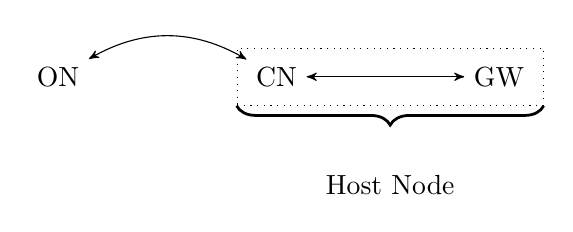
\begin{tikzpicture}[node/.style={circle,draw}]
      \begin{scope}[node distance=2cm]
        \node (a) {ON};
        \node (b) [right=of a] {CN};
        \node (c) [right=of b] {GW};
      \end{scope}

      \begin{scope}[<->,>=stealth',auto]
        \path (a) edge[bend left] (b)
        (b) edge (c);
      \end{scope}

      \node[draw,dotted,fit=(b)(c)](group){};
      \draw[line width=1pt,black,decorate,decoration={amplitude=7pt,brace,mirror}]
      (group.south west) -- (group.south east);
      \node[below=of group,anchor=center]{Host Node};

  \end{tikzpicture}
  \caption{Architecture of a \fitlab node in the testbed}
  \label{fig:fitnode}
\end{figure}

\subsection{The Open Node}

The \ac{ON} is either based on the
\emph{WSN430}\footnote{\url{https://www.iot-lab.info/hardware/wsn430/}}, an
\emph{M3}\footnote{\url{https://www.iot-lab.info/hardware/m3/}} or an
\emph{A8}\footnote{\url{https://www.iot-lab.info/hardware/a8/}} microprocessor,
and a different number of nodes of each type are available depending on the test
site. All nodes except the \emph{A8} node can run \emph{RIOT}
\cite{baccelli2013riot}, \emph{OpenWSN} \cite{watteyne2012openwsn},
\emph{FreeRTOS}\footnote{\url{http://www.freertos.org/}} and \emph{Contiki},
The \emph{A8} only supports
Linux. In addition, the \emph{WSN430}
also has support for \emph{TinyOS} \cite{levis2005tinyos}. Some of the nodes are
mobile and can be configured to move on specified paths through the network.
Their movements can be tracked using \ac{GPS} and are available to the user.

In this evaluation, the \emph{M3} node has been selected for use as the \ac{ON}.
(see \autoref{subsubsec:reasonsm3}).

\subsection{The M3 Node}
\label{subsec:m3}

All experiments in this work have been performed using the \emph{M3} open node.
A simplified block diagram of this node can be seen in
\autoref{fig:m3node}\footnote{\url{https://github.com/iot-lab/iot-lab/wiki/Hardware_M3-node}}.
None of the external peripherals are used in the experiment and can therefore be
disabled to conserve energy.

\begin{figure}
  \centering
  \begin{tikzpicture}
    \node[processor] (cpu)[minimum width=50,minimum height=50] {M3}; %STM32F103RKEY

    \node[memory] (flash) [below of=cpu,below=0.5] {Flash}; %N25Q128A
    \draw[bus,transform canvas={xshift=-10}] (flash) edge node[buslabel] {GPIO} (cpu);
    \draw[bus,transform canvas={xshift=10}] (flash) edge node[buslabel] {SPI} (cpu);

    \node[radio] (wireless) [right of=cpu,above of=cpu,right=0.4] {Radio}; %AT86RF231
    \path[bus] (wireless.240) |- node[buslabel,above] {GPIO} (cpu.10);
    \path[bus] (wireless) |- node[buslabel] {SPI} (cpu);

    \node[system] (usbb) [above of=cpu,above=1] {USB Bridge};
    \path[bus] (usbb) edge node[buslabel] {JTAG} (cpu);
    \path[bus,transform canvas={xshift= 20}] (usbb) edge node[buslabel] {UART} (cpu);

    \node[connector] (oc) [above of=usbb,above=1,minimum width=100] {Open Node Connector};
    \path[bus] (usbb) edge node[buslabel]{USB} (oc) ;
    \path[bus] (oc.190) |- node[buslabel]{GPIO} (cpu.160) ;

    \node[connector] (usb) [right of=oc,below of=oc,right=0.5] {USB};
    \path[bus] (oc) |- (usb);

    \node[processor] (pm) [below of=usb] {Power};

    \node[sensor] (light)   [minimum width=80,below left of=oc,left=1.5] {Light Sensor}; %ISL29020
    \node[sensor] (pressure)[minimum width=80,below of=light] {Pressure Sensor}; %LPS331AP
    \node[sensor] (gyro)    [minimum width=80,below of=pressure] {Gyroscope}; %L3G4200D
    \node[sensor] (magneto) [minimum width=80,below of=gyro] {Magnetometer}; %LSM303DLHC

    \path[bus] (oc.188) |- (light);
    \path[bus] (oc.188) |- (gyro);
    \path[bus] (oc.188) |- (magneto);
    \path[bus] (oc.188) |- (pressure);
    \path[bus] (oc.188) |- node[buslabel,below] {I2C} (cpu.190);
    \path[bus] (gyro)   -| node[buslabel,below] {GPIO} (cpu.120);
    \path[bus] (magneto.10)-| (cpu.120);

    \path[vcc] (pm.210) |- node[below] {+3.3 V} (usbb);
    \path[vcc,orange,text=black] (pm) -- node[auto] {+3.3 V mon.} (wireless);
    \path[vcc] (usb) -- node[left] {+5} (pm);
    \path[vcc] (oc.340) |- node[near start,auto] {+3.3} (pm.165);
    \path[vcc,orange,text=black] (oc.330) |- node[near start,left] {+5} (pm.175);

    \path[vcc,orange,text=black] (pm) |- (1,1.8) -| (cpu.70);
    \path[vcc,orange,text=black] (pm) |- (1,1.8) -- (0.5,1.8);
    \node[rounded rectangle,right of=pm,right=0.1] (gnd) {GND};
    \path[vcc,<->] (pm) -- (gnd);

  \end{tikzpicture}
  \caption{Simplified block diagram of the M3 node}
  \label{fig:m3node}
\end{figure}

% better than wsn430: more diversity, closer to real world deployments in modern iot

\subsubsection{CPU}

The \emph{M3} node features a 32-bit ARM Cortex-M3 based CPU (STM32F103REY)
\cite{stm32f103re} with a maximum clock frequency of 72 MHz. The external clock
runs the \ac{CPU} at this maximum clock frequency, which is to be considered
when evaluating the energy consumption. With all peripherals enabled, this
results in a maximum of 70 mA at 3.3 V \ac{VCC}.

The \ac{CPU} has support for low power modes. When in the \emph{Sleep} mode, the
\emph{CPU} is stopped and all peripherals continue working, in the \emph{Stop}
mode all clocks are stopped and only the contents of \ac{SRAM} and \ac{CPU}
registers are preserved. When in the \emph{Standby} mode the contents of the
registers and \emph{SRAM} are not preserved and the \emph{CPU} can only be woken
up by alarms from the \ac{RTC} or an external reset.

The \ac{JTAG} and \ac{UART} are bridged over \ac{USB} and exposed through the
\emph{Open Node Connector}.

\subsubsection{Flash Memory}

The external \emph{N25Q128} \cite{N25Q128} NOR flash is connected to the
\ac{SPI} of the \ac{CPU} and has a storage capacity of 128 MByte and supports a
maximum frequency of 100 MHz. The \ac{CPU} uses a maxium of 18 MHz for the
\ac{SPI} which results in a maximum 18 Mb/s read / write speed. The
current consumption for page size read / write access is 20 mA.

\subsubsection{Wireless Radio Transceiver}

The \emph{M3} has an ATMEL AT86RF231 2.4 GHz radio \cite{AT86RF231}, which is
connected through \ac{SPI} and \ac{GPIO} and are supplied with 3.3 V. It consumes up to
14 mA when transmitting with a maximum \ac{TX} gain of 3 dBm. For this work, the
\ac{TX} has been set to -7 dBm and the \ac{RX} threshold has been set to -60 dBm
(see \autoref{subsec:rssi}). As such, \ac{TX} needs less than 11 mA when transmitting and
10 mA while receiving. The \emph{6LowPAN} network \cite{rfc4944} stack of \emph{Contiki}
uses the IEEE 802.15.4 support of the transceiver.

\subsubsection{Rationale for Choosing the M3 Node}
\label{subsubsec:reasonsm3}

Instead of the \emph{WSN430}, the \emph{M3} node has been selected for the
evaluation. While the \emph{WSN430} has the advantage of having almost the same processor
(\emph{MSP430}) as the \emph{Z1} node, driver support for the \emph{WSN430}
peripherals like the NOR Flash is based on an an outdated version of
\emph{Contiki}. Moreover, only a very limited amount of nodes of this type had
been available at the time of writing and also not in the linear topology
desirable for the evaluation \autoref{sec:ptopo}.

While the drivers for the \emph{M3} do not support energy estimations using
\emph{Energest} \cite{dunkels2011powertrace}, in-case of the \emph{M3} node,
\emph{Host Node} can record the voltage, current and power consumption of the
\ac{ON} in real time. In doing so, even more accurate and realistic measurements
of the energy consumption are available compared to the profiling done using
\emph{Powertrace}. The \emph{WSN430} for one is not controlled by the \emph{Host
Node} so not all variables that would be desirable for the evaluation, such as
\ac{PCAP} files, can be recorded with it.

Another reason for selecting the \emph{M3} node instead of the \emph{WSN430}
was, that a more powerful processor is available, as will likely be the case in
most modern \ac{IoT} applications, and as such it better models the energy
consumption of these use-cases.

\subsubsection{Considerations for Power Consumption}
One thing to keep in mind when measuring the power consumption at the \ac{ON} is
that only the consumption of the components that can be controlled by the
firmware is monitored. For this, the power management unit monitors the voltage
and current of a separate output besides the one supplying the \ac{USB} bridge. The
power management unit can be supplied both through the open node connector (3.3
V) or directly via \ac{USB} (+5 V).

The core components, on which the experiments in this work have an effect in
terms of power consumption,, are the flash memory, because of the persistence
layer for \ac{RPL}, the \ac{CPU} because the restoring needs some amount of
cycles to complete and the radio, as additional / fewer routing messages may be
sent in the individual modes of the hardened implementation.

The peripheral components, such as the different sensors are not of interest for
the evaluation, since they are not differently depending on whether there are
resets occurring or if the hardened implementation is being used.

\begin{table}
  \centering
  \caption{Consumption estimates for monitored components}
  \begin{tabular}{lr}
    \toprule
    Component & Current Consumption (3.3 V) \\
    \midrule
    CPU & 70 mA \\
    Radio & SLEEP 20 $\mu$A | OFF 0.4 mA | RX 10.3 mA | TX 10 mA\\
    Flash & 20 mA 
  \end{tabular}
  \label{tab:consum}
\end{table}

\autoref{tab:consum} shows the different consumption estimates as they were
obtained from the data sheets of the components. It should be noted, that the
consumption of the \ac{CPU} and the wireless radio could be further reduced by
reducing the clock rate the \ac{CPU} is initialized with and reducing the
transmission power of the radio. Both can be configured using software. For the
evaluation, it was sufficient to keep these values, since a relative comparison
between networks with and without resets should be made.

\subsection{Host Node}

For the \emph{M3} and \emph{A8} nodes, the \ac{HN} serves as both the \ac{GW}
and the \ac{CN}. Each \ac{HN} is directly connected to one or more \ac{ON} using
the \emph{Open Node Connector} and serves the purpose of controlling and
recording the experiment on the \ac{ON}. A simplified block diagram of the
\emph{Host Node} is shown in \autoref{fig:hnblock}.

The \ac{CN} is used for starting and stopping the \ac{ON}, flashing the firmware
and providing a remote \ac{JTAG} debugger via the \ac{USB} bridge on the \ac{ON}
and powering the \ac{ON} from battery or the an external power supply. It also
can monitor the power consumption and record the \ac{RSSI} at the \ac{ON}. As an
alternative to monitoring the \ac{RSSI} the \ac{CN} can record \acp{PCAP} of the
network at the \ac{ON}. For this it has its own radio, similar to the one
supplying the \emph{M3} \ac{ON}. It can also be used for recording sensor data from the
peripherals of the \ac{ON} using \ac{I$^2$C}.

The \ac{GW} part of the \ac{HN} features a more powerful \emph{A8} application
processor and is connected to the site server using a wired
\emph{Ethernet} connection. It is running \emph{Linux} and can provide the
\ac{HN} with network access for applications such as running a remote debugger,
flashing the firmware and starting and stopping the node. It also stores the
measured data from the \ac{CN} which then periodically is fetched by the
site server.

Both the \ac{CT} and the \ac{AM} of the power management unit are configurable
in the profile of the experiment so that a range of different \ac{PM} can be
used for sampling the consumption.

\begin{equation}
  PM = CT \times AM \times 2
\end{equation}

\begin{figure}
  \pgfdeclarelayer{background}
  \pgfdeclarelayer{foreground}
  \pgfsetlayers{background,main,foreground}

  \centering

  \begin{tikzpicture}
    % CN part

    \node[processor] (cpu)[minimum width=50,minimum height=50] {M3};
    \node[radio] (wireless) [right of=cpu,right=0.5] {Radio};
    \node[system] (bridge) [below of=cpu,below=0.5] {USB Bridge};

    \path[bus] (bridge.120) -- node [buslabel,left] {JTAG} (cpu.260);
    \path[bus] (bridge.60) -- node [buslabel,right] {SPI} (cpu.280);

    \path[bus] (wireless.north west) -- node [buslabel,above] {SPI} (cpu.19);
    \path[bus] (wireless.south west) -- node [buslabel,below] {GPIO} (cpu.-19);

    \begin{pgfonlayer}{background}
      \node [draw,fit=(cpu)(wireless)(bridge),label=above:\tiny{Control Node},fill=tubsGray20] (cn) {};
    \end{pgfonlayer}

    \node[processor] (a8) [minimum width=100,minimum height=100,left of=cn,left=4,above of=cpu] (a8) {A8};
    \node[system] (eth) [below of=a8,below=1] {ETH SW};
    \node[connector] (eth0) [below of=eth,right of=eth,below=0.001] {ETH};
    \node[connector] (eth1) [below of=eth,below=0.001] {ETH};
    \node[connector] (eth2) [below of=eth,left of=eth,below=0.001] {ETH};
    \path[bus] (eth) -- node[buslabel,above] {ETH} (a8);
    \path[bus] (eth1) -- (eth);
    \path[bus] (eth0) |- (eth);
    \path[bus] (eth2) |- (eth);

    \node[system] (uhub) [above of=a8,above=2,left of=a8] {USB Hub};
    \path[bus] (uhub) -- node[buslabel,below] {USB} (a8.120);

    \node[connector] (usb0) [above of=uhub] {USB};
    \node[connector] (usb1) [above of=uhub,left of=uhub] {USB};
    \node[connector] (usb2) [above of=uhub,right of=uhub] {USB};
    \path[bus] (usb2) |- (uhub);
    \path[bus] (usb0) -- (uhub);
    \path[bus] (usb1) |- (uhub);

    \node[system] (ubridge2) [right of=uhub,right=2,above of=a8,above=1] {USB Bridge};
    \path[bus] (ubridge2) -- node[buslabel,below] {UART} (a8.60);

    \node[connector] (onc) [minimum width=200,right of=usb2,right=0.5] {Open Node Connector};

    \node[connector] (pwr) [right of=onc,right=3] {Power};

    \node[processor] (pwrmgnt) [below of=pwr,below=1] {Power Mgnt};

    \node[processor] (cmsr) [below of=pwrmgnt,left of=pwrmgnt,left=2] {Current Msr};

    \path[bus] (ubridge2) |- node[buslabel] {USB} (onc.south west);
    \path[bus] (eth.north east) -| node[buslabel] {ETH} (onc.187);
    \path[bus] (bridge.north west) -| node[buslabel] {UART} (onc.190);
    \path[bus] (cpu.160) -| node[buslabel,left] {GPIO} (onc.192);
    \path[bus] (cpu.north west) -| node[buslabel,right] {I2C} (onc.194);

    \path[vcc,<-] (usb2.south east) |- (3.55,4) -- (pwrmgnt.north west);
    \node[label=above left:\tiny{5V}] at (3.55,4) {};
    \path[vcc] (3.55,4) -| (cmsr.100);
    \path[vcc] (pwrmgnt.north west) -- (onc.south east);
    \path[vcc] (pwr) -- node[buslabel,right] {+3.3V to 5V} (pwrmgnt);
    \path[vcc,<->] (cmsr.north east) |- (pwrmgnt);
    \path[vcc] (pwrmgnt) |- node[buslabel] {+48V} (4.5,-2.4) -| (eth0.east);

    \path[vcc,orange] (pwrmgnt.160) |- (onc.east);
    \path[vcc,orange] (pwrmgnt.160) |- node[buslabel,below] {+3.3V} (1,3.5) -- (cmsr.28);

    \node[draw,rounded rectangle] (gnd) at (2.8,2) {GND};
    \path[vcc] (gnd) |- (pwrmgnt);
  \end{tikzpicture}
  \caption{Simplified block diagram of the Host Node}
  \label{fig:hnblock}
\end{figure}

\section{Physical Topology of the Testbed}
\label{sec:ptopo}

When looking at previous studies, the influence of the physical topology of a
network on the routing topology came to attention. This can be used to
affect the routing decisions of \ac{RPL} and reliably create certain \acp{DAG}
in some cases. Nevertheless, with such a large test network of linearly
distributed, we can study the full range of possible outcomes resulting from
\ac{RPL} being applied to it.

For the evaluation, a large network of 44 nodes that are approximately linearly
distributed inside the test lab has been selected. A map of the test network at
\emph{Inria}\footnote{\url{https://www.iot-lab.info/deployment/lille/}} in
France is shown in \autoref{fig:testbed}, where the red nodes are selected for
our experiment, the grey nodes are mounted at the ceiling over a 1.2 $\times$
1.2 m grid at a height of 2.5 m, yellow nodes are attached to vertical poles at
2.4 m, 1.5 m and 0.6 m high and the green square represents the position of the
server cabinet. Additionally, the floor-plan is shown as an outline.

Nodes participating in the experiment are marked as blue circle. Node \emph{157}
has been statically selected as the root of the \ac{DAG}.

\tikzstyle{cnode}=[circle,fill=tubsLightOrange100,text centered,font=\tiny,fill
opacity=0.5,draw opacity=0.5,text opacity=1.0]
\tikzstyle{snode}=[circle,fill=tubsGray20,text centered,font=\tiny,fill
opacity=0.2,draw opacity=0.2,text opacity=1.0]
\tikzstyle{pnode}=[circle split,draw,text centered,fill=tubsLightOrange20,draw opacity=0.1,text opacity=1.0,fill opacity=0.1,font=\tiny]

%TODO latex number vs strings wtf

\newcommand{\fitnode}[3]{%
  \ifthenelse
  {#3 = 47 \OR #3 = 49 \OR #3 = 51 \OR #3 = 53 \OR #3 = 57 \OR #3 = 59 \OR #3 = 83 \OR #3 = 85 \OR #3 = 87 \OR #3 = 89 \OR #3 = 91 \OR #3 = 93 \OR #3 = 95 \OR #3 = 123 \OR #3 = 127 \OR #3 = 131 \OR #3 = 133 \OR #3 = 151 \OR #3 = 153 \OR #3 = 155 \OR #3 = 157 \OR #3 = 159 \OR #3 = 161 \OR #3 = 192 \OR #3 = 194 \OR #3 = 196 \OR #3 = 198 \OR #3 = 200 \OR #3 = 202 \OR #3 = 204 \OR #3 = 218 \OR #3 = 220 \OR #3 = 222 \OR #3 = 224 \OR #3 = 226 \OR #3 = 228 \OR #3 = 230 \OR #3 = 244 \OR #3 = 246 \OR #3 = 248 \OR #3 = 250 \OR #3 = 252 \OR #3 = 254 \OR #3 = 256}%\isin{47}{ \OR #3 = 47 \OR #3 = 49 \OR #3 = 51 \OR #3 = 53 \OR #3 = 57 \OR #3 = 59 \OR #3 = 83 \OR #3 = 85 \OR #3 = 87 \OR #3 = 89 \OR #3 = 91 \OR #3 = 93 \OR #3 = 95 \OR #3 = 123 \OR #3 = 127 \OR #3 = 131 \OR #3 = 133 \OR #3 = 151 \OR #3 = 153 \OR #3 = 155 \OR #3 = 157 \OR #3 = 159 \OR #3 = 161 \OR #3 = 192 \OR #3 = 194 \OR #3 = 196 \OR #3 = 198 \OR #3 = 200 \OR #3 = 202 \OR #3 = 204 \OR #3 = 218 \OR #3 = 220 \OR #3 = 222 \OR #3 = 224 \OR #3 = 226 \OR #3 = 228 \OR #3 = 230 \OR #3 = 244 \OR #3 = 246 \OR #3 = 248 \OR #3 = 250 \OR #3 = 252 \OR #3 = 254 \OR #3 = 256}}
  {\node at (#1,#2) [cnode] {#3};}
  {\node at (#1,#2) [snode] {#3};}
}

\begin{figure}
  \centering

  \usetikzlibrary{shapes}

  \begin{tikzpicture}
    \draw [black!20] (-0.3,13) -- (7.5,13) -- (7.5,4.8) -- (8.7,4.8) -- (8.7,0.8) -- (4.2,0.8) -- (4.2,-0.6) -- (-0.3,-0.6) -- cycle;
    \draw [tubsBlack!20] (8.7,13) -- (13.2,13) -- (13.2,-0.6) -- (8.7,-0.6) -- cycle;
    \fill [tubsLightGreen] (4.7,12.4) rectangle (5.3,12.9);
    \fill [tubsBlack!20] (-0.3,9.2) rectangle (-0.2,11.9);
    \fill [tubsBlack!20] (-0.3,0.2) rectangle (-0.2,2.6);
    \fill [tubsBlack!20] (0,13) rectangle (2.2,13.1);
    \draw [tubsBlack!20] (-0.4,3.95) rectangle (-0.3,4.1);
    \draw [tubsBlack!20] (-0.4,7.95) rectangle (-0.3,8.10);
    \draw [tubsBlack!20] (4.05,3.75) rectangle (4.2,3.9);
    \draw [tubsBlack!20] (4.05,8.05) rectangle (4.2,8.2);
    \draw [tubsBlack!20] (7.40,8.05) rectangle (7.55,8.2);
    \draw [tubsBlack!20] (8.65,3.75) rectangle (8.80,3.9);
    \foreach \x in {0,1,...,4} {
      \foreach \y in {0,1,...,12} {
        \pgfmathparse{int(29+\x*18+(12-\y))}
        \edef\p{\pgfmathresult}
        \fitnode{\x}{\y}{\p}
      }
    }
    \foreach \x in {0,1,...,2} {
      \foreach \y in {1,2,...,12} {
        \pgfmathparse{int(123+\x*14+(12-\y))}
        \edef\p{\pgfmathresult}
        \fitnode{\x+5}{\y}{\p}
      }
    }
    \foreach \y in {1,2,...,7} {
      \pgfmathparse{int(190-\y)}
      \edef\p{\pgfmathresult}
      \fitnode{8}{\y}{\p}
    }
    \foreach \y in {9,10,...,12} {
      \pgfmathparse{int(191-\y)}
      \edef\p{\pgfmathresult}
      \fitnode{8}{\y}{\p}
    }
    \foreach \x in {0,1,...,4} {
      \foreach \y in {0,1,...,12} {
        \pgfmathparse{int(256-(4-\x)*13-\y)}
        \edef\p{\pgfmathresult}
        \fitnode{\x+9}{\y}{\p}
      }
    }
    \foreach \y in {0,2,...,24} {
      \pgfmathparse{int(25-\y)}
      \edef\p{\pgfmathresult}
      \pgfmathparse{int(\p+1)}
      \edef\q{\pgfmathresult}
      \node at (-0.3,\y/2) [pnode] {\p \nodepart{lower} \q};
    }
    \node at (0,13) [pnode] {27 \nodepart{lower} 28};
    \node at (1,13) [pnode] {45 \nodepart{lower} 46};
    \node at (2,13) [pnode] {63 \nodepart{lower} 64};
    \node at (3,13) [pnode] {81 \nodepart{lower} 82};
    \node at (4,13) [pnode] {99 \nodepart{lower} 100};
    \node at (0,-1) [pnode] {42,43 \nodepart{lower} 44};
    \node at (1,-1) [pnode] {60,61 \nodepart{lower} 62};
    \node at (2,-1) [pnode] {78,79 \nodepart{lower} 80};
    \node at (3,-1) [pnode] {96,97 \nodepart{lower} 98};
    \node at (4,-1) [pnode] {114,115 \nodepart{lower} 116};
    \node at (4.3,0.8) [pnode] {\nodepart{lower} 121,122};
    \node at (5,0.8) [pnode] {\nodepart{lower} 135,136};
    \node at (6,0.8) [pnode] {\nodepart{lower} 149,150};
    \node at (7,0.8) [pnode] {\nodepart{lower} 163,164};
    \node at (8,0.8) [pnode] {\nodepart{lower} 190,191};
    \foreach \y in {0,2,4,6,8} {
      \pgfmathparse{int(177-\y)}
      \edef\p{\pgfmathresult}
      \pgfmathparse{int(\p+1)}
      \edef\q{\pgfmathresult}
      \node at (7.5,\y/2+5) [pnode] {\p \nodepart{lower} \q};
    }
    \foreach \y in {12,14} {
      \pgfmathparse{int(179-\y)}
      \edef\p{\pgfmathresult}
      \pgfmathparse{int(\p+1)}
      \edef\q{\pgfmathresult}
      \node at (7.5,\y/2+5) [pnode] {\p \nodepart{lower} \q};
    }
    \node at (4.2,3.9) [pnode] {\nodepart{lower} 119,120};
    \node at (4.2,8.1) [pnode] {117,118};
  \end{tikzpicture}
  \caption{Positions of nodes inside the Lille testbed}
  \label{fig:testbed}
\end{figure}

\subsection{Radio Distances and RSSI}
\label{subsec:rssi}

Another important consideration when selecting the number of nodes has been the
distance between the nodes. When performing preliminary testing on the formation
of the network, it has been observed that the network quickly broke down after a
larger number of nodes had been started. By default, the \ac{RX} threshold and
the \ac{TX} power of each nodes radio transceiver are configured to such values
that all nodes are within radio distance of each other. When the network starts
up, each node attempts to announce its presence to its neighbors using
\ac{ICMPv6} messages. With the selected number of nodes this causes a sufficient
number of collisions for the back-off procedure of \emph{ContikiMAC} to fail and
thus no messages can be transmitted successfully.

For such a problem, multiple resolutions can be thought of including increasing
the distance between the nodes, reducing the number of nodes and reducing
\ac{TX} power and increasing the \ac{RX} threshold. Since the positions
of the nodes are fixed and the area of the test lab is limited, increasing the
distance between the nodes is not an option. Reducing the number of nodes would
decrease the size of the resulting routing topology, which also is not
desirable. In this case, it has been sufficient to follow the recommended
method\footnote{\url{https://github.com/iot-lab/iot-lab/wiki/Limit-nodes-connectivity}}
for controlling node connectivity and to reduce the transmission gain from 0 dBm
to -3 dBm and increase the sense threshold from -101 dBm to -60 dBm.

\subsection{Maintenance Status of Nodes}

The status of all nodes inside the test lab can be viewed using the \ac{API} of
\fitlab. When observing the set of available nodes, a significant amount of
nodes was not available for experimentation and marked as \emph{down}, which
amounted for about half of all nodes.

\section{Accessing to the Testbed}

\fitlab offers programmable interfaces for setting up and controlling
experiments, and obtaining the results. These interfaces are accessible over the
internet using either the \ac{REST}-\ac{API}. Measurement results can be
obtained through \ac{SSH} from a server that is located at the site. The
different interfaces are depicted in \autoref{fig:access}.

\begin{figure}
  \centering
  \usetikzlibrary{fit}
  \begin{tikzpicture}
    \node (U) at (0,0) [shape=circle,draw,fill=tubsLightGreen20] {User};
    \node (A) at (3,0) [fill=tubsLightOrange20,shape=rounded rectangle,draw] {API};
    \node (S) at (6,0) [fill=tubsLightOrange20,shape=rectangle,draw] {Site Server};
    \path (U) edge [arrows=<->,auto,swap] node {REST} (A);
    \path (U) edge [arrows=<->,bend left] node [auto,swap] {SSH} (S);
    \path (A) edge [arrows=<->] (S);
    \node (n1) at (8.5,-1) [fill=tubsLightBlue20,shape=ellipse,draw] {HN};
    \node (n2) at (8.5,0) [fill=tubsLightBlue20,shape=ellipse,draw] {HN};
    \node (n3) at (8.5,1) [fill=tubsLightBlue20,shape=ellipse,draw] {HN};
    \foreach \n in {n1,n2,n3} \path (\n) edge [arrows=<->,auto,swap] (S);
    \path (A) edge [arrows=<->] (S);
    \begin{pgfonlayer}{background}
      \node [label=above:Intranet,fill opacity=0.2,shape=rounded rectangle,fill=tubsLightViolet80,fit=(n1)(n2)(n3)(S)] {};
      \node [label=below left:Internet,fill opacity=0.2,shape=rounded rectangle,fill=tubsLightBlue80,fit=(U)(A)(S)] {};
    \end{pgfonlayer}
  \end{tikzpicture}
  \caption{Accessing the testbed}
  \label{fig:access}
\end{figure}

\subsection{REST API}

The \ac{REST} \ac{API} is provided by an \ac{HTTP} server that and can access
all site servers and as such can send commands to and query all \ac{HN} at
each side. This section describes methods of \ac{API} that have been used in the
experiments.

The \ac{API} for controlling experiments supports the creation and deletion of
experiments. All previous experiments can be queried for a description of their
settings and resources. Also, the state of each experiment can be monitored.
Each configuration of an experiment includes a unique number by which the
experiment will be identified, a list of resources (e.g. firmwares) and nodes.
Each experiment also includes an association of each node with a firmware file
and a profile.

Profiles are managed independently of experiments, although for each experiment a
different profile can be selected. Profiles describe how the \ac{HN} of a node
will be configured during the experiment. These settings include the whether the
node will be powered from battery of from an external power supply, the settings
for the current measurement unit, and the settings for monitoring the radio of
the \ac{CN}.

New firmware files can be uploaded through the \ac{API} and flashed to either a
selection of nodes or all nodes associated with the experiment. This way it is
possible to assign different firmwares for the \ac{DAG} root and all other
nodes.

\subsection{Site Server}

At each site, a central server takes care of coordinating all nodes
participating in an experiment. It is accessed by the \ac{API} for executing the
functions it exposes through the its \ac{REST} interface. Besides through the
\ac{API}, the site server can also be accessed directly using \ac{SSH}. Both the
server and each \ac{HN} are part of the same \emph{Ethernet} network and
communicate using \ac{TCP}/\ac{IP}.

Measurement data is periodically collected from the different \ac{HN} and stored
inside the home directory of the user running the associated experiment. This
data can then be transferred or examined by the user by executing commands on
the server.
